% https://tex.stackexchange.com/a/762399/322482
% https://tex.stackexchange.com/questions/583318/multi-colored-edges-in-tikz-undirected-graph/688634#688634
\documentclass[tikz,border=5pt]{standalone}
\usetikzlibrary{arrows.meta,bending,nfold}
\makeatletter
\tikzset{
  foo/.tip={Stealth[harpoon,swap]},
  mystyle/.style={thick,shorten >=2pt,shorten <=2pt},
  offset/.code=
    \tikz@addoption{%
      \pgfgetpath\tikz@temp
      \pgfsetpath\pgfutil@empty
      \pgfoffsetpath\tikz@temp{#1}
    },
  dualharpoon/.style={
    draw=none,
    postaction={path only,draw,foo-,mystyle,offset=+.3ex},
    postaction={path only,draw,-foo,mystyle,offset=-.3ex}
  }
}
\makeatother
\begin{document}
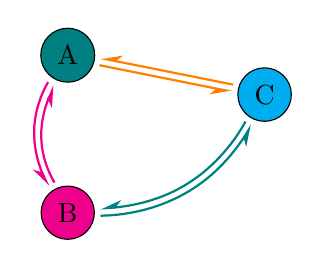
\begin{tikzpicture}
    \node[draw,circle,fill=teal] (A) at (0,1) {A};
    \node[draw,circle,fill=magenta] (B) at (0,-1) {B};
    \node[draw,circle,fill=cyan] (C) at (2.5,.5) {C};
    \draw[dualharpoon,magenta] (A) to[bend right] (B);
    \draw[dualharpoon,teal] (B) to[bend right] (C);
    \draw[dualharpoon,orange] (A) -- (C);
\end{tikzpicture}
\end{document}
